
% !TEX TS-program = XeLaTeX
% !TEX encoding = UTF-8 Unicode

\documentclass[border=10pt]{standalone}

\usepackage[dvipsnames]{xcolor}	    % Load before tikz
\usepackage[hidelinks]{hyperref}
\usepackage{tikz, tkz-euclide} 
\usepackage{qcircuit}

\usepackage{fontspec}
\usepackage[OT1]{fontenc}

\usepackage{eulervm} 				% Load before amssymb
\usepackage{amsmath}
\usepackage{amssymb}


\IfFontExistsTF{Trump Mediaeval LT Std}{%
	\setromanfont[Mapping=tex-text, Scale=0.95, AutoFakeSlant]{Trump Mediaeval LT Std}
}

\overfullrule=1mm

\newcommand{\thetitle}{On the Weyl chamber of Canonical 2-qubit quantum gates}
\hypersetup{ 
	pdfauthor={Gavin E. Crooks}, 
	pdftitle={\thetitle} ,
}

\newcommand{\Gate}[1]{{\sf{#1}}}

\begin{document}


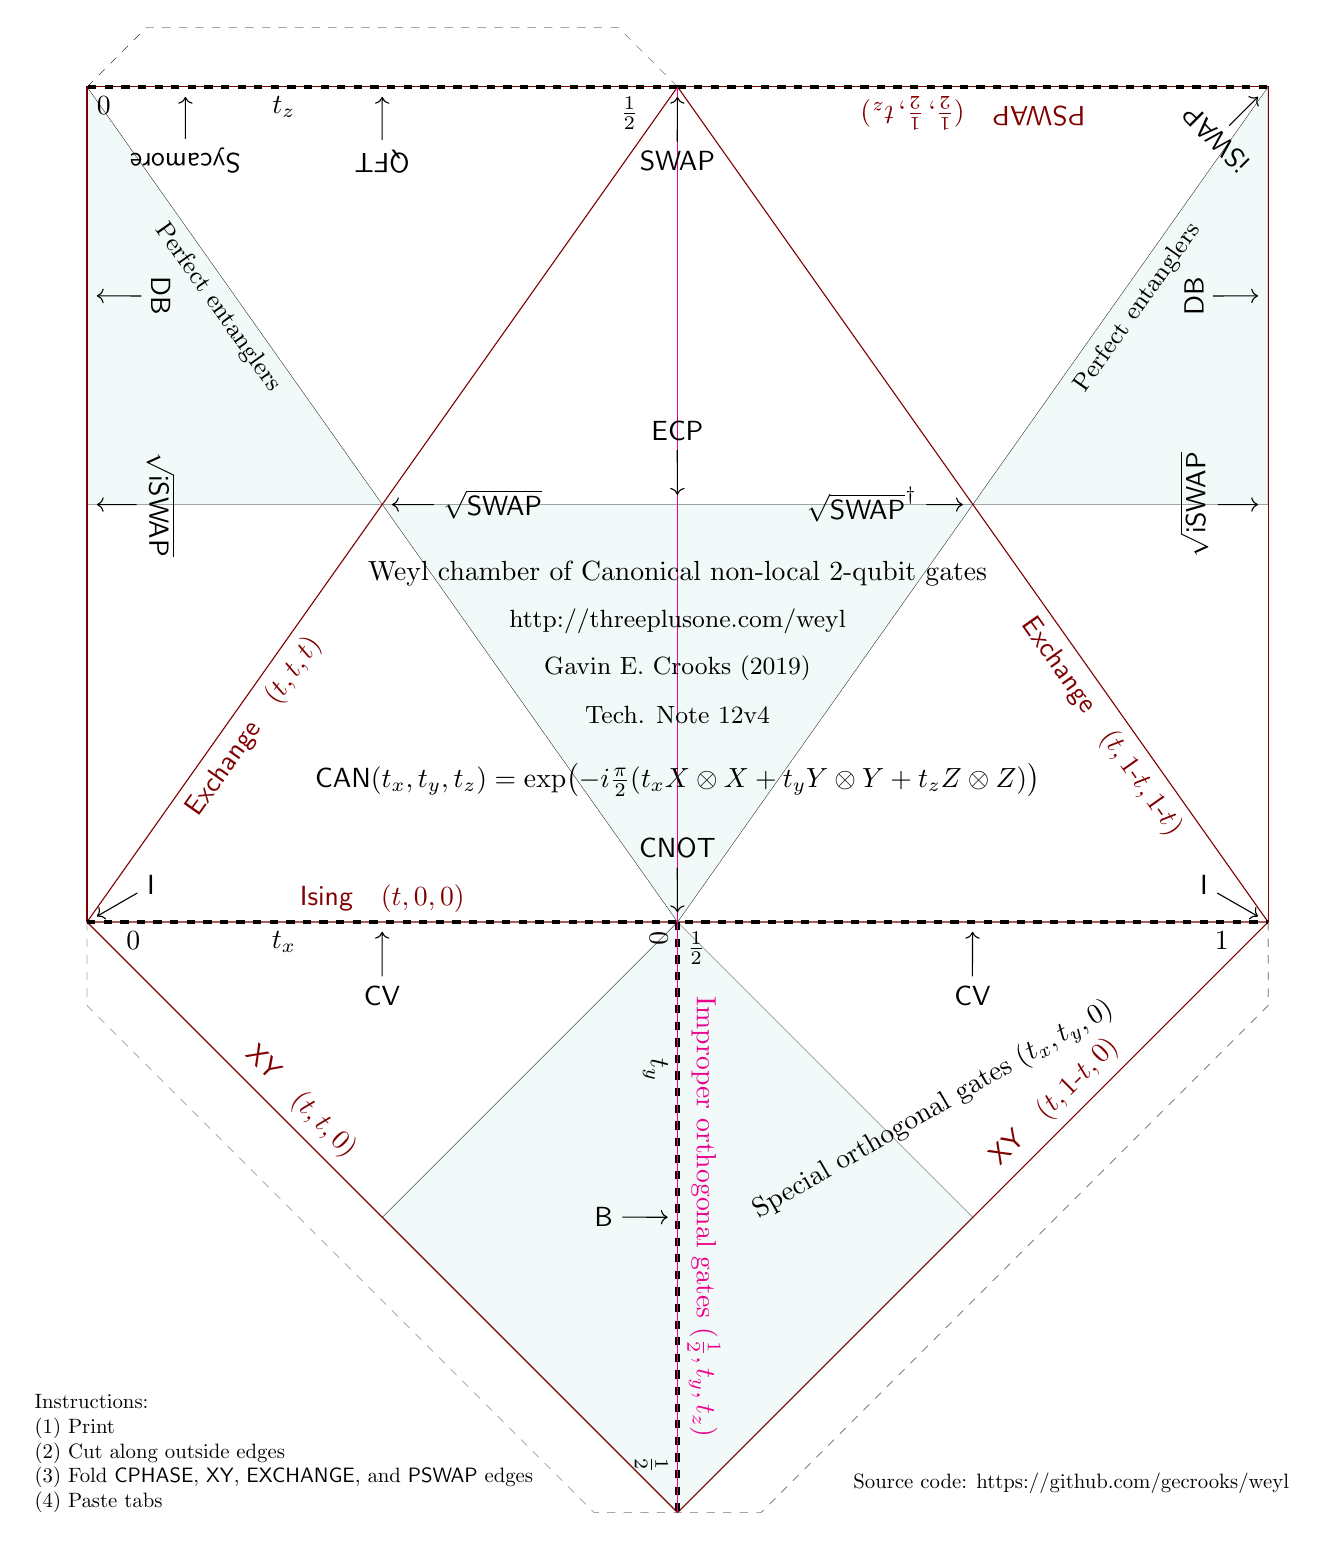
\begin{tikzpicture}[scale=7.5]

\def\sep{0.125}  % Separation between gates and gate labels
\def\ang{54.74} % = arctan(sqrt(2)) in degrees, angle of EXCHANGE line 


% Perfect entanglers
\draw [ultra thin, fill=teal!5] (1, 0) -- ({1/2}, {sqrt(2)/2}) -- ({3/2}, {sqrt(2)/2}) -- (1, 0);
\draw [ultra thin, fill=teal!5] (0, {sqrt(2)}) -- ({1/2}, {sqrt(2)/2}) -- (0, {sqrt(2)/2}) -- (0, {sqrt(2)});
\draw [ultra thin, fill=teal!5] (2, {sqrt(2)}) -- ({3/2}, {sqrt(2)/2}) -- (2, {sqrt(2)/2}) -- (2, {sqrt(2)});
\draw [ultra thin, fill=teal!5] (1, 0) -- ({1/2}, {-1/2}) -- (1, -1) --   ({3/2}, {-1/2}) -- (1, 0);

\node [below, rotate=-\ang] at ({1/4}, {sqrt(2)*3/4}) {\small{Perfect entanglers}};
\node [below, rotate= \ang] at ({7/4}, {sqrt(2)*3/4}) {\small{Perfect entanglers}};



% Draw boundary
\draw [Maroon] (0,0) -- (2, 0) -- (1,-1) -- (0,0); 					% Bottom triangle
\draw [Maroon] (0,0) -- (1, {sqrt(2)}) -- (2, 0); 					% Top triangle
\draw [Maroon] (0,0) -- (0, {sqrt(2)}) -- (2, {sqrt(2)}) -- (2,0);	% Upper rectangle


% Draw tabs
\def\tabsize{0.1};					
\draw [ultra thin, dashed] (0, {sqrt(2)}) 
						-- (0 + \tabsize, {sqrt(2) + \tabsize}) 
						-- (1 - \tabsize, {sqrt(2) + \tabsize})
						-- (1, {sqrt(2)});
\draw [ultra thin, dashed] (0, 0) 
						-- (0, {0 - sqrt(2) * \tabsize}) 
						-- ({1 - sqrt(2) * \tabsize}, -1)
						-- (1, -1);
\draw [ultra thin, dashed] (2, 0) 
						-- (2, {0 - sqrt(2) * \tabsize}) 
						-- ({1 + sqrt(2) * \tabsize}, -1)
						-- (1, -1);



% Axes
\draw [dashed, ultra thick] (0, 0) -- (2, 0);
\draw [dashed, ultra thick] (1, {sqrt(2)}) -- (0, {sqrt(2)});
\draw [dashed, ultra thick] (1, {sqrt(2)}) -- (2, {sqrt(2)});
\draw [dashed, ultra thick] (1, 0) -- (1, -1);

\node [below right] at (0+0.05, 0) {$0$};
\node [below] at ({1/3}, 0) {$t_x$};
\node [below right] at (1, 0) {$\tfrac{1}{2}$};
\node [below left] at (2-0.05, 0) {$1$};

\node [below right, rotate=-90] at (1, 0) {$0$};
\node [below, rotate=-90] at (1, -{1/4}) {$t_y$};
\node [below left, rotate=-90] at (1, -1+0.05) {$\tfrac{1}{2}$};

\node [below right] at (0, {sqrt(2)}) {$0$};
\node [below] at ({1/3}, {sqrt(2)}) {$t_z$};
\node [below left] at (1-0.05, {sqrt(2)}) {$\tfrac{1}{2}$};


%% Gate families

% Orthogonal gates
\draw [ultra thin, magenta] (1,0) -- (1, {sqrt(2)});
\draw [ultra thin, magenta] (1,0) -- (1, -1);
\node [above, rotate=-90, magenta] at (1, -{1/2}) {Improper orthogonal gates $(\tfrac{1}{2}, t_y, t_z)$};
\node [above, rotate=30] at ({0.1+ 1+sqrt(2)/4}, -{sqrt(2)/4}) {Special orthogonal gates $(t_x, t_y, 0)$};

% CPHASE
\node [above, Maroon] at ({1/2}, 0) {$\Gate{Ising}\quad(t,0,0)$};

% XY
\node [above, Maroon, rotate=-45] at ({1/3}, {-1/3}) {$\Gate{XY}\quad(t,t,0)$};
\node [above, Maroon, rotate=45] at ({2-1/3}, {-1/3}) {$\Gate{XY}\quad(t,1$-$t,0)$};

% EXCHANGE
\node [below, Maroon, rotate=\ang] at ({1/4}, {sqrt(2)/4}) {$\Gate{Exchange}\quad(t,t,t)$};
\node [below, Maroon, rotate=-\ang] at ({2-1/4}, {sqrt(2)/4}) {$\Gate{Exchange}\quad(t,1$-$t,1$-$t)$};

% PSWAP
\node [above, Maroon, rotate=180] at ({3/2}, {sqrt(2)}) {$\Gate{PSWAP}\quad(\tfrac{1}{2},\tfrac{1}{2},t_z)$};



%% Gate Nodes
\node (I) 		at (0, 0) {};
\node (I_L) 	at ([shift={(30:\sep)}]I) {\Gate{I}};
\draw [->] (I_L) -- (I);

\node (I2) 		at (2, 0) {};
\node (I2_L) 	at ([shift={(150:\sep)}]I2) {\Gate{I}};
\draw [->] (I2_L) -- (I2);

\node (CNOT) 	at (1, 0) {};
\node (CNOT_L) 	at ([shift={(90:\sep)}]CNOT) {\Gate{CNOT}};
\draw[->] (CNOT_L) -- (CNOT);

\node (SWAP) 	at (1, {sqrt(2)}) {};
\node (SWAP_L) at ([shift={(270:\sep)}]SWAP) {$\Gate{SWAP}$};
\draw[->] (SWAP_L) -- (SWAP);

\node (SWAPR) 	at ({1/2}, {sqrt(2)/2}) {};			% Root of SWAP
\node (SWAPR_L) at ([shift={(0:{\sep*3/2})}]SWAPR) {$\sqrt{\Gate{SWAP}}$};
\draw[->] (SWAPR_L) -- (SWAPR);

\node (SWAPRI) 	at ({3/2}, {sqrt(2)/2})	{};			% SWAP, Sqrt, inverse
\node (SWAPRI_L) at ([shift={(180:{\sep*3/2})}]SWAPRI) {$\sqrt{\Gate{SWAP}}^\dagger$};
\draw[->] (SWAPRI_L) -- (SWAPRI);

\node (ECP)		at (1, {sqrt(2)/2}) {};
\node (ECP_L) at ([shift={(90:\sep)}]ECP) {${\Gate{ECP}}$};
\draw[->] (ECP_L) -- (ECP);

\node (B)		at (1, {-1/2}) {};
\node (B_L) at ([shift={(0:-\sep)}]B) {${\Gate{B}}$};
\draw[->] (B_L) -- (B);

\node (ISWAP) at (0, {sqrt(2)}) {};
\node (ISWAP2)	at (2, {sqrt(2)}) {};
\node [rotate=135] (ISWAP2_L) at ([shift={(225:\sep)}]ISWAP2) {${\Gate{iSWAP}}$};
\draw[->] (ISWAP2_L) -- (ISWAP2);

\node (ISWAPR)	at (0, {sqrt(2)/2}) {};
\node [rotate=270] (ISWAPR_L) at ([shift={(0:\sep)}]ISWAPR) {$\sqrt{\Gate{iSWAP}}$};
\draw[->] (ISWAPR_L) -- (ISWAPR);

\node (ISWAPR2)	at (2, {sqrt(2)/2}) {};
\node [rotate=90] (ISWAPR2_L) at ([shift={(180:\sep)}]ISWAPR2) {$\sqrt{\Gate{iSWAP}}$};
\draw[->] (ISWAPR2_L) -- (ISWAPR2);

\node (DB) at (0, {sqrt(2)*3/4}) {};
\node [rotate=270] (DB_L) at ([shift={(0:\sep)}]DB) {${\Gate{DB}}$};
\draw[->] (DB_L) -- (DB);

\node (DB2) at (2, {sqrt(2)*3/4}) {};
\node [rotate=90] (DB2_L) at ([shift={(180:\sep)}]DB2) {${\Gate{DB}}$};
\draw[->] (DB2_L) -- (DB2);

\node (QFT)		at ({1/2}, {sqrt(2)}) {};
\node [rotate=180] (QFT_L) at ([shift={(270:\sep)}]QFT) {${\Gate{QFT}}$};
\draw[->] (QFT_L) -- (QFT);

\node (QFT2) at ({3/2}, {sqrt(2)}) {};

\node (SYC)		at ({1/6}, {sqrt(2)}) {};
\node [rotate=180] (SYC_L) at ([shift={(270:\sep)}]SYC) {${\Gate{Sycamore}}$};
\draw[->] (SYC_L) -- (SYC);


\node (CNOTR) at ({1/2}, 0) {};
\node (CNOTR_L) at ([shift={(270:\sep)}]CNOTR) {$\Gate{CV}$};
\draw[->] (CNOTR_L) -- (CNOTR);

\node (CNOTR2)	at ({3/2}, 0) {};
\node (CNOTR2_L) at ([shift={(270:\sep)}]CNOTR2) {$\Gate{CV}$};
\draw[->] (CNOTR2_L) -- (CNOTR2);


\node at (1, 0.59){Weyl chamber of Canonical non-local 2-qubit gates};
\node at (1, 0.51){\small{\url{http://threeplusone.com/weyl}}};
\node at (1, 0.43){\small{Gavin E. Crooks (2019)}};
\node at (1, 0.35){\small{Tech. Note 12v4}};


\node at (1,0.24){$\Gate{CAN}(t_x, t_y, t_z)  = \exp\bigl(-i\frac{\pi}{2}
	(t_x X\otimes X + t_y Y\otimes Y + t_z Z \otimes Z) \bigr)$};


\node[align=left, scale=0.75] at ({1/3}, -0.9) {
	Instructions:\\
	(1) Print\\
	(2) Cut along outside edges\\
	(3) Fold \Gate{CPHASE}, \Gate{XY}, \Gate{EXCHANGE}, and \Gate{PSWAP} edges\\
	(4) Paste tabs
};

\node[align=left,, scale=0.75] at ({5/3}, -0.95) {Source code: \url{https://github.com/gecrooks/weyl}};


\end{tikzpicture}


\end{document}
